% Chapter 
\chapter{Pragmatics} % Write in your own chapter title
\label{Chapter6}
%\lhead{Chapter 5. \emph{Pragmatics}} % Write in your own chapter title to set the page header
%\section{Introduction}
In this chapter, I discuss the pragmatic effects associated with the attachment of certain verbal prefixes, mentioned in the previous chapter. The main aim of the Sections~\ref{sec:pragm:old}, \ref{sec:pragm:tests}, and \ref{sec:pragm:new} is to establish that, contrary to most analyses, the inferences associated with the perfective aspect of the derived verb and particular verbal prefixes are not semantic presuppositions. 

In Section~\ref{sec:pragm:old}, I explore two common claims. The first claim is that perfective verbs trigger a presupposition that the initial phase (or the process part) of events denoted by them actually took place (henceforth a \textit{process presupposition}). While exploring this claim, I outline the evidence in favour of a semantic presuppositional analysis offered in previous Slavic studies and provide a brief overview of an alternative pragmatic approach, proposed by \citet{Gronn:04, Gronn:06}.

The second claim is that there is a presupposition triggered by specific verbal prefixes independently of the grammatical properties of the whole surface verb. The prefixes that are discussed in this respect are the completive prefix \textit{do-} and the repetitive prefix \textit{pere-}. These prefixes have been claimed to give rise to presuppositions similar to those associated with lexical items like \textit{finish} and \textit{again}, respectively (see \citealt{Kagan:book} and Sections~\ref{subsection:semantics:pere}--\ref{subsection:semantics:do} here).

Section~\ref{sec:pragm:tests} presents evidence against the presuppositional approach outlined in Section~\ref{sec:pragm:old}. In Section~\ref{sec:pragm:new}, I show that both cases of inferences (related to the perfective aspect and to the prefixes \textit{do-} and \textit{pere-}) are better analysed as scalar implicatures in negative contexts and questions and as entailments in affirmative declarative sentences. This hypothesis is supported by empirical tests that allow to tease apart presuppositions, entailments and (scalar) implicatures associated with Slavic verbs. The testing methodology relies on some results from recent research in the domain of projective content (\citealp{Schlenker:08, Chemla:09, Romoli:11}, and references therein). Sections~\ref{sec:pragm:old}--\ref{sec:pragm:new} present joint work with Hana Filip, also published as \citealt{ZinovaFilip:SALT} and \citealt{ZinovaFilip:14}. %In those sections \textit{we} refers to Hana Filip and myself. 

The last section of this chapter, Section~\ref{section:pragm:overall}, is dedicated to providing an overall picture of how the whole prefixation system works when the range of meanings available for the prefixed verbs gets constrained by pragmatic competition. 

\section{Previous approaches}\label{sec:pragm:old}
\subsection{Inferences associated with the perfective aspect}\label{sec:pragm:old:perf}
This section addresses the common claim that perfective verbs presuppose the initial phase (or a process part) of the events denoted by them, and assert their final phase (or a culmination part), while the meaning of imperfective verbs lacks both these components. Different formulations of this claim have been proposed by \citet{Paducheva:96, Paducheva:11} and \citet{Romanova:06} for Russian, and by \citet{Docekal:09} for Czech.

As an example, consider \ref{ex:pos:pro}. It contains a perfective verb \textit{pro\v{c}itat'} `to read through' that denotes (a set of) accomplishments (its imperfective simplex base \textit{\v{c}itat'} `to read' denotes (a set of) processes). According to the proposals by \citet{Paducheva:96, Paducheva:11}, \citet{Romanova:06}, and \citet{Docekal:09}, \ref{ex:pos:pro} presupposes the existence of the process (initial) part of events it denotes, i.e., `Ivan started reading the book' and asserts that the denoted events culminated, i.e., `Ivan finished reading the book'.

\exg.\label{ex:pos:pro}Ivan pro\v{c}ital$^{\PF}$ \`{e}tu knigu.\\
Ivan pro.read.\glb{pst}.\glb{sg.3} this book\\
\trans `Ivan read this book completely through.'

The presuppositional nature of the process component of perfective verbs is viewed as being confirmed by the observation that it is preserved under negation and in questions, as shown in \ref{2-a} and \ref{2-b}, respectively: 

\ex.\label{2}\ag.\label{2-a}Ivan ne pro\v{c}ital$^{\PF}$ \`{e}tu knigu.\\
Ivan not pro.read.\glb{pst}.\glb{sg.m} this book\\
\trans `Ivan did not read this book completely through.'\\
\textit{Assertion:} Ivan did not finish reading this book.\\
\textit{Inference:} Ivan started reading/read a part of this book.
\bg.\label{2-b}Ivan pro\v{c}ital$^{\PF}$ \`{e}tu knigu?\\
Ivan pro.read.\glb{pst}.\glb{sg.m} this book\\
\trans `Has/Did Ivan read this book completely through?'\\
\textit{Question:} The speaker asks the addressee to confirm or deny whether Ivan finished reading this book.\\
\textit{Inference:} Ivan started reading/read a part of this book.

In the example \ref{2-a} the meaning component that is negated is the culmination, but not the process (initial) part of described events, i.e., \ref{2-a} can be felicitously uttered in a situation in which it is known that Ivan started reading the book. In \ref{2-b}, what is questioned is whether the speaker finished reading the book. To the extent that the previous studies rely on the negation and question tests, it is fair to assume that what they have in mind is a semantic presupposition. The presence of a presupposition is sometimes \citep[e.g., by][]{Paducheva:96, Romanova:04} also viewed as a common core of all perfective verbs. Let us now address the details of the analyses that follow from different linguistic traditions.

%However, not all the perfective verbs contain prefixes, one example is the pair \textit{re\v{s}at'$^{IPF}$ -- re\v{s}it'$^{\PF}$} `to decide, to solve.' The claim above address all perfective accomplishments, independently of the means they were formed with. The verb \textit{pro\v{c}itat'} with a specific prefix \textit{pro-} is only taken as an illustration of a perfective verb that does not significantly differ in its semantics from the corresponding imperfective verb. In the precious studies such pairs as \textit{\v{c}itat'} -- \textit{pro\v{c}itat'} and \textit{re\v{s}it'} -- \textit{re\v{s}at'} are called \textit{aspectual pairs} \citep[see, e.g.,]{Forsyth:70} and prefixes that participate in the formation of perfective verbs in aspectual verbs are often called \textit{empty prefixes}, or \textit{\v{c}istovidovyje pristavki} in Russian tradition, (see \citealp{Saxmatov:52, Shvedova:82} for traditional view and \citealp{EndersenJanda:12} for arguments against the existence of empty prefixes). On the other hand, the completive prefix \textit{do-} and the iterative prefix \textit{pere-} that are discussed in connection with the second claim each have specific significant semantic contribution (this contribution is also regular and such prefixes are commonly called \textit{superlexical} as opposed to \textit{lexical prefixes}, whose semantic contribution is non-regular and non-compositional, see \citealp{Babko-Malaya:99, Svenonius:04a, Ramchand:04}, among many others).

\subsubsection{Russian linguistic tradition}
In the Russian linguistic tradition, the idea that perfective verbs have a bipartite structure can be traced back to Maslov (1984). On his view, Russian perfective verbs consist of an ``eventive'' part \textit{(sobytijnyj komponent)} and a ``stative / resultative'' part \textit{(statal'nyj komponent}).

Building on Maslov (1984), \citet{Paducheva:96, Paducheva:11} proposes that these two components of perfective verbs differ in their communicative status. What roughly corresponds to Maslov's `eventive' component is presupposed and concerns backgrounded information. On her view, it comprises not only the process part of events described by perfective verbs, but also their preparatory conditions and various pragmatic factors like intentions, expectations and obligations associated with the utterance of sentences headed by perfective verbs. The second, asserted, component regards focused information, including the `reaching of a/the boundary', i.e., the final phase of events involving goals, results, and limits of various sorts. 

Padu\v{c}eva (1996) illustrates these points by contrasting sentences \ref{3-a} and \ref{3-b}. According to her, the sentence \ref{3-a}, which is headed by an imperfective verb, is a neutral question about whether a cab was called. Sentence \ref{3-b}, which is headed by a perfective verb, in addition suggests that from the point of view of the speaker the addressee was required, expected, or obliged to call a cab. 

\ex.\label{3}\ag.\label{3-a}Taksi vyzyvali$^{\IPF}$?\\
Taxi call.\glb{pst}.\glb{pl}\\
\trans `Did you call a cab?'\Source{= (1a) in \citealt[55]{Paducheva:96}}
\bg.\label{3-b}Vy vyzvali$^{\PF}$ taksi?\\
you.\glb{pl} call.\glb{pst}.\glb{pl} taxi\\
\trans `Did you call a cab?'\\
\textit{Presupposition}: The hearer was expected/required to call a cab.\\\Source{= (1a) in \citealt[55]{Paducheva:96}}

Although \citet{Paducheva:96} adduces a number of valid and subtle intuitions in support of her approach to the uses of perfective verbs (e.g., the negation test), as opposed to imperfective ones, its major weakness is that it fails to separate between the semantic meaning components of perfective verbs,  and various speech-act-related pragmatic inferences (such as speaker's deontic and normative expectations on the addressee) associated with utterances of sentences with perfective verbs. 
 
The second problem, and one that is also mentioned in \citealt{Gronn:04}, is that the observed speaker-oriented modality inferences are not consistently attached to all the uses of sentences with perfective verbs. For instance, as \citet{Gronn:04} observes, they are not associated with the utterances of affirmative sentences headed by perfective verbs. Take, for example, \ref{4}, which is an affirmative correspondent of \ref{3-b}, but unlike \ref{3-b} does not suggest (under the most neutral circumstances) that the referent of \textit{ja} `I' was required, expected, or obliged to call a cab:

\exg.\label{4}Ja vyzval$^{\PF}$ taksi.\\
 I call.\glb{pst}.\glb{sg.m} taxi\\
 \trans `I called a cab.'\Source{= example (53) in \citealt[61]{Gronn:04}}
 
\citet[56]{Paducheva:96} also observes that there is no reason to assume that the utterance of \ref{4} triggers the inference of an ``expectation component'' (``komponent o\v{z}idanija'') on the part of the speaker, but she does not motivate this observation any further. That is, Padu\v{c}eva (1996) is aware of the fact that not all the sentences with perfective verbs carry the relevant inference (or ``presupposition'' in her wide sense), but she does not provide any account when it may, must or must not be present in sentences with perfective verbs. 
 
\subsubsection{Syntactic approaches to the decomposition of perfective verbs}
Following \citet{Paducheva:96}, \citet{Romanova:06} proposes that ``perfective verbs must have a complex semantic structure, where one part is asserted, the other is presupposed'' (p.~29). She adopts the characterisation of the presupposed part given by \citet{Paducheva:96}, but has a different understanding of the asserted component. 

 Most importantly, according to \citet{Romanova:06}, ``it is not true that only resultative verbs or the verbs with `reaching-the-boundary' component, can bear the presupposition of perfectives'' (p.~29), but rather all perfectives are ``words that encode decomposable structures (informational, semantic and therefore syntactic)'' (ibid., p.~53). For example, even the class of inceptive verbs like those with the prefix \textit{za}-  (e.g., \textit{zapet'} `to begin to sing') which fail to entail culmination or result of some sort (under the most usual understanding), are taken to have a complex semantic structure, whereby the first part is presupposed. According to \citet{Romanova:06}, the sentence \ref{5}, for instance, asserts that Tonja did not start to sing and presupposes that Tonja was expected to sing her song.
 
\exg.\label{5}Tonja ne zapela$^{\PF}$ svoju pesnju.\\
Tonja not za.sing.\glb{pst}.\glb{sg.f} self's.\glb{f.acc} song.\glb{acc}\\
\trans `Tonja didn't start to sing her song.'\\
\textit{Presupposition:} Tonja was expected to sing her song.\\\Source{= example (64a) in \citealt[29]{Romanova:06}}

Another example that is used by \citet{Romanova:06} is provided under \ref{6} here: the sentence is claimed to be associated with a presupposition that the addressee was suppposed to buy bread.

\exg.\label{6}Ty kupila$^{\PF}$ xleb?\\
You.\glb{sg.nom} bought.\glb{pst}.\glb{sg.f} bread.\glb{acc}\\
\trans `Did you buy bread?'\\
\textit{Presupposition}: You were supposed to buy bread.\\
\Source{= example (65) in \citealt[30]{Romanova:06}}

This generalisation allows \citet{Romanova:06} to represent the semantics of all perfective verbs as that of accomplishments, which are commonly assumed to have a bipartite structure. \citet{Romanova:06} follows a syntactic approach of \citet{Ramchand:04}, on which accomplishments are analysed in terms of syntactic structures that consist of two separate projections, namely process (ProcP) and result (resP). Those projections correspond to the presuppositional and assertive components of the meaning of perfective verbs, respectively. 

There are three main problems with the account by \citet{Romanova:06}. First, the meaning of perfective verbs as a whole class cannot be assimilated to that of accomplishments \citep[for counterarguments see][]{Filip:00, FilipRothstein:05}. Obviously, there are perfective verbs that cannot be meaningfully decomposed into two subevents, a process and a result subevent. One good example is the class of semelfactive verbs with the suffix \textit{-nu-} in Russian, such as \textit{prygnut'} `to jump'. 

 Second, what remains entirely unclear is the representation of speaker- and/or addressee-oriented attitudes in terms of syntactic structures. For instance, the syntactic representation of the alleged `contrary to the expectation' (see example \ref{5}) and obligation (see example \ref{6}) inference that is supposed to be associated with the process (ProcP) part of the syntactic structure of perfective verbs remains on a pretheoretic level.

 Third, it is easy to show that the alleged presuppositional meaning components (here, the expectation of the speaker on the addressee or on some participant of the situation described by perfective sentences) are not tied to the uses of perfective verbs only, which is a point of criticism that also applies to the proposal of \citet{Paducheva:96}. Compare \ref{5} with \ref{7}. Sentence \ref{5} is headed by a perfective verb, while sentence \ref{7} is headed by the corresponding imperfective simplex verb. Also \ref{7}, and not only \ref{5}, triggers the inference that Tonja was expected to sing her song.

\exg.\label{7}Tonja ne pela$^{\IPF}$ svoju pesnju.\\
 Tonja not sing.\glb{pst}.\glb{f.sg} self's.\glb{f.acc} song.\glb{acc}\\
 \trans `Tonja wasn't singing/didn't sing her song.'\\
\textit{Inference:} Tonja was expected to sing her song.

The account proposed by \citet{Romanova:06} also inherits the problems related with the proposal of \citet{Paducheva:96}: first, the failure to distinguish between semantic components of perfective verbs and pragmatic factors having to do with obligations, expectations and the like on the part of the interlocutors, and second, the fact that the alleged presuppositions of perfective verbs fail to be present in all their uses, most notably in utterances of affirmative sentences. 

\subsubsection{Event semantics}
One illustrative example of an event semantics approach is \citet{Docekal:09}. They take it for granted that all perfective verbs have a uniform meaning of telic predicates. Telic predicates are equated with accomplishment predicates, which means that they are decomposed into two subevents, where e$_1$ is a process and e$_2$ is the result state \citep[mainly following][]{Giorgi:01}. Their main innovation is the claim that perfective verbs carry the ``activity presupposition'' tied to e$_1$ or ``the first homogeneous part of telic events''. The evidence for this claim comes from the observation that it exhibits the usual projective properties of a semantic presupposition: namely, it ``projects under negation and under a question operator''.

Similar to the case of the proposal by \citet{Romanova:06}, an immediate problem with this account is that the meaning of perfective verbs as a whole class cannot be equated with that of accomplishments. Another problem is noticed by \citet{Docekal:09} themselves: namely, imperfective verbs can also carry the ``activity presupposition''. A case in point is the class of secondary imperfective verbs (in most cases explicitly marked with the imperfective suffix \textit{-yva-}) that are formed with the ``completive'' (or ``terminative'') prefix \textit{do-}, as in the example \ref{8-a}. The sentence \ref{8-a} denies that Vasya was about to finish reading the book yesterday, and implies that he read a part of it, but was nowhere near being close to finishing reading it. But notice that the same inference -- namely that Vasya read a part of the book -- is also triggered by the sentence with the corresponding perfective verb \ref{8-b}:

\ex.\label{8}\ag.\label{8-a}V\v{c}era Vasja ne do\v{c}ityval$^{\IPF}$ tu knigu.\\
Yesterday Vasya not do.read.\glb{imp}.\glb{pst}.\glb{sg.m} that book\\
\trans `Yesterday Vasya was not finishing reading that book.'\\
\textit{Inference}: He started reading that book.
\bg.\label{8-b}V\v{c}era Vasja ne do\v{c}ital$^{\PF}$ tu knigu.\\
Yesterday Vasya not do.read.\glb{pst}.\glb{sg.m} that book\\
\trans `Yesterday Vasya did not finish reading that book.'\\
\textit{Inference}: He started reading that book.

\citet{Docekal:09} acknowledge that such prefix usages as the terminative usage of the prefix \textit{do-}, when they constitute a part of a secondary imperfective verb, are problematic for their account, because secondary imperfectives with such prefixes can also trigger the ``activity presupposition'' just like perfective verbs. They set this problem aside for future research. 

\subsubsection{Summary of the presuppositional accounts}
All the works summarised up to this point share the claim that all and only perfective verbs can be decomposed into two parts, effectively having the bipartite structure of accomplishments. In this bipartite structure, the first part (`process' or `activity') is presupposed while the second part (`result') is asserted. However, there is a number of perfective verbs that do not have the structure of accomplishments, i.e., that cannot be plausibly decomposed into a process and a result component \citep[see][and references therein]{Filip:00, FilipRothstein:05}. 

 Second, some studies of perfective verbs \citep[here represented by][]{Paducheva:96, Romanova:06} contain claims about the association of perfective verbs with certain speaker-oriented modalities; particularly prominent are speaker's normative and deontic expectations on the addressee. Such speech-act-related factors clearly lie outside of the lexical semantic structure of perfective verbs (which is not to deny that they may arise from the interaction of the lexical meaning of perfective verbs with pragmatic factors). This raises the question about the distribution and robustness of such pragmatic inferences that are allegedly associated with the uses/meaning of perfective verbs. 

 Third, despite frequent claims about the `presupposition' of perfective verbs, there seems to be little reflection on the status of such claims, and if any concrete empirical evidence is adduced at all, it is their preservation under negation and in questions. However, not all that projects is a presupposition \citep[see, e.g.,][]{ChierchiaMcConnell-Ginet:90, Beaver:01, Potts:05}, so more evidence is needed to establish the status of the observed inferences.

\subsubsection{Pragmatic implicature}
\citet[61]{Gronn:04} correctly recognises that ``[t]he negation test in itself is not a sufficient argument for associating perfective accomplishments with a presupposition''. Instead, he proposes that the process inference is a matter of pragmatic implicature \citep{Grice:75}.

The account by \citet{Gronn:04, Gronn:06} is based on two main assumptions. First, it relies on the markedness theory of Slavic aspect \citep{Maslov:58, Jakobson:71}, according to which the imperfective aspect is semantically unmarked, i.e., unspecified with respect to the distinguishing semantic feature of the perfective
aspect that is taken to be the marked member of the aspectual opposition.
Second, it integrates pragmatic assumptions related to speaker's and hearer's economy effort in communication, based on ``the Gricean idea that the best form-meaning pairs are the ones which minimize both the speaker's and hearer's effort (whose interests are, in a sense, conflicting)'' \citep[][71]{Gronn:06}. \citeauthor{Gronn:06}'s idea of aspectual competition can be illustrated with the following examples:

\ex.\ag.\label{ex:negimp}Ivan ne \v{c}ital$^{\IPF}$ \`{e}tu knigu.\\
Ivan not read.\glb{pst}.\glb{sg.3} this book\\
\trans `Ivan did not read this book.'
\bg.\label{ex:negpf}Ivan ne pro\v{c}ital$^{\PF}$ \`{e}tu knigu.\\
Ivan not pro.read.\glb{pst}.\glb{sg.3} this book\\
\trans `Ivan did not read this book completely through.'\\\Source{= ex.~\ref{2-a} in this chapter}

The unmarked imperfective \ref{ex:negimp} is the default choice of the speaker when the existence of a whole (culminated) event is negated.
If the speaker chooses \ref{ex:negpf}, with the aspectually marked perfective form, instead of the unmarked imperfective one, as in \ref{ex:negimp}, the hearer infers that there was some attempt or activity on the part of the agent of the described events which did not culminate, because it would have been more economic for the speaker to use the unmarked imperfective, if it were possible/relevant.

This account is implemented in Optimality Theory \citep{Blutner:00} and provides an important contribution to the understanding of aspectual distinction in Russian due to the shift from semantic presupposition to pragmatic analysis.

\subsection{Prefixes: The completive \textit{do-} and iterative \textit{pere-}}\label{sec:pragm:old:pref}
The completive prefix \textit{do-} is claimed to behave similarly to the English verb \textit{finish}. For example, \citet[75]{Kagan:book} states that ``\textit{finish} and \textit{do-} presuppose that a particular event begins, or takes place partially, and entail that it reaches a certain finishing point''. As an illustration, consider \ref{ex:pos:do} that contains a perfective verb \textit{do\v{c}itat'} `to finish reading', formed with the completive prefix \textit{do-}. According to \citet{Kagan:book}, the sentence in \ref{ex:pos:do} entails that the whole book was read and presupposes that the event of reading the book took place.

\ex.\ag. \label{ex:pos:do}Ivan do\v{c}ital$^{\PF}$ \`{e}tu knigu.\\
Ivan do.read.\glb{pst}.\glb{sg.3} this book\\
\trans `Ivan finished reading this book.'
\bg. \label{ex:pos:pere}Ivan pere\v{c}ital$^{\PF}$ \`{e}tu knigu.\\
Ivan pere.read.\glb{pst}.\glb{sg.3} this book\\
\trans `Ivan reread this book.'

As for the iterative prefix \textit{pere-}, \citet[145]{Kagan:book} states that \ref{ex:pos:pere} ``presupposes that Ivan read the book in question before the event time and entails that another reading event took place''. Note that the prefix \textit{pere-} has a range of other meanings (see Section~\ref{subsection:semantics:pere}) that are irrelevant here.

In support of a presuppositional analysis, \citet{Kagan:book} relies on the negation test. The negation of \ref{ex:pos:do}, shown in \ref{ex:neg2}, is claimed to presuppose that Ivan read a part of the book and to negate the culmination of the reading event. The sentence in \ref{ex:neg3} is taken to presuppose that Ivan read the book before and negate the existence of the second completed reading event.

\ex.\ag.\label{ex:neg2}Ivan ne do\v{c}ital$^{\PF}$ \`{e}tu knigu.\\
Ivan not do.read.\glb{pst}.\glb{sg.3} this book\\
\trans `Ivan did not finish reading this book.'\\
\textit{Inference}: Ivan read a part of this book.
\bg. \label{ex:neg3}Ivan ne pere\v{c}ital$^{\PF}$ \`{e}tu knigu.\\
Ivan not pere.read.\glb{pst}.\glb{sg.3} this book\\
\trans `Ivan did not reread this book.'\\
\textit{Inference}: Ivan read this book before.

If perfective accomplishments prefixed with the completive prefix \textit{do-} and the iterative prefix \textit{pere-} are tested, as is done in \citealt{Kagan:book} and also illustrated here by the examples \ref{ex:neg2} and \ref{ex:neg3}, two different phenomena are potentially confounded. Specifically, if the completive \textit{do-} constitutes a part of a complex perfective verb, its contribution overlaps with the meaning of perfective aspect. In order to eliminate the confounding factor of perfectivity and to get at the semantics of these two prefixes, it is better to test them when they occur in imperfective verbs, i.e., when they co-occur with the secondary imperfective suffix and no other prefix(es) on the same verb.

%It must be noted here that as long as the question about the nature of the inferences triggered by perfective aspect is not completely solved, it has to be clearly separated from the question about the inferences associated with specific prefixes. If perfective accomplishments prefixed with the completive prefix \textit{do-} and the iterative prefix \textit{pere-} are tested, as is done in \citet{Kagan:11} and illustrated by examples \ref{ex:neg2}, \ref{ex:neg3}, \ref{ex:q2}, and \ref{ex:q3}, potentially two different phenomena are mixed. Specifically, if the completive \textit{do-} constitutes a part of a complex perfective verb, its contribution overlaps with the meaning of perfective aspect. So in this section we are going to test verbs that contain either the completive prefix \textit{do-} or the iterative prefix \textit{pere-} (and no other prefixes) and the secondary imperfective suffix. Such verbs are imperfective, so the inference associated with perfective aspect of the verb does not intervene in this case.

To illustrate that the question about presupposition triggering arises at all in the case of imperfective verbs containing the prefixes \textit{do-} and \textit{pere-}, let us address the examples in \ref{ex:imperf}. As shown,  \ref{ex:imperf1} has an inference that the reading of the book started and \ref{ex:imperf2} has an inference that there was a previous event of reading (either completed or not).

\ex.\label{ex:imperf}\ag.\label{ex:imperf1}Ivan ne do\v{c}ityval$^{\IPF}$ \`{e}tu knigu.\\
Ivan not do.read.\glb{pst}.\glb{sg.3} this book\\
\trans `Ivan did not finish/was not finishing reading this book.'\\
\textit{Inference}: Ivan read a part of this book.
\bg.\label{ex:imperf2}Ivan ne pere\v{c}ityval$^{\IPF}$ \`{e}tu knigu.\\
Ivan not pere.read.\glb{pst}.\glb{sg.3} this book\\
\trans `Ivan did not reread/was not rereading this book.'\\
\textit{Inference}: Ivan read/was reading this book before.

\section{Evidence against a presuppositional approach}\label{sec:pragm:tests}
The account by \citet{Gronn:04, Gronn:06} summarised above sheds considerable doubts on the status of the inferences in question as semantic presuppositions. Therefore, in this section, I take a closer look at them, relying on standard tests used in the research on projective meaning to diagnose semantic and pragmatic presuppositions, in particular in contrast with scalar implicatures. These tests provide evidence that the process inference associated with perfective verbs is not a matter of either semantic or pragmatic presupposition. The same tests are also applied to test the status of inferences triggered by the completive prefix \textit{do-} and the iterative prefix \textit{pere-}. However, they do not lead to any conclusive results in this case.
\subsection{Projection out of the antecedents of conditionals}
According to theories of presupposition projection, semantic presuppositions project out of the antecedents of conditionals, as in \ref{ex:pres}, but scalar implicatures do not \ref{ex:si}.

\ex.\a.\label{ex:pres:neg}John didn't win the marathon.\\
$\rightarrow$ John participated in the marathon.
\b.\label{ex:pres}If John won the marathon, he will celebrate tonight.\\
$\rightarrow$ John participated in the marathon.
\b.\label{ex:pres:cond:neg}If John didn't win the marathon, he will not celebrate tonight.\\
$\rightarrow$ John participated in the marathon.

The sentence \ref{ex:pres:neg} contains a presupposition trigger: the verb \textit{to win}. Under negation, the inference that John participated in the marathon is preserved. It is also preserved when the same trigger is located in the antecedent of a conditional, both in affirmative, as in the sentence \ref{ex:pres}, or negated, as in the sentence \ref{ex:pres:cond:neg}, variants.
\ex.\a.\label{ex:si:neg}John didn't read all the books.\\
$\rightarrow$ John read some of the books.
\b.\label{ex:si}If John read all the books, he will pass the exam.\\
$\nrightarrow$ John read some of the books.
\b.\label{ex:si:cond:neg}If John didn't read all the books, he will fail the exam.\\
$\nrightarrow$ John read some of the books.

If, instead of the presupposition trigger \textit{to win}, a scalar item such as \textit{all} is used, the inference under negation, as in the sentence \ref{ex:si:neg}, seems to be of the same kind as in \ref{ex:pres:neg}. However, examples that involve conditionals reveal the difference between the inferences that arise due to the presuppositional triggers and inferences that arise due to the presence of the scalar items. For instance, in \ref{ex:si} and \ref{ex:si:cond:neg} the inference that John read some of the books no longer projects.

Now let us explore the Russian data. Example \ref{ex:cond} shows that the alleged ``process presupposition'' that is claimed to be triggered by perfective accomplishments does not project out of the antecedents of conditionals. Hence, it fails to exhibit one of the properties of semantic presupposition.

\exg.\label{ex:cond}Esli Vasja pro\v{c}ital$^{\PF}$ u\v{c}ebnik, on sdast \`{e}kzamen.\\
if Vasya pro.read.\glb{pst}.\glb{sg.m} textbook he passes exam\\
\trans `If Vasya completely read the textbook, he will pass the exam.'\\
$\nrightarrow$ Vasya read/began reading the textbook.

As far as the prefixes \textit{do-} and \textit{pere-} are concerned, native speakers have no clear intuitions as to whether the alleged inferences in \ref{ex:cond:do} and \ref{ex:cond:pere}, which are traditionally taken to be of presuppositional nature, hold. Recall that in order to separate the contribution of prefixes from perfective aspect, it is better to test their contribution in imperfective verbs.

\exg.\label{ex:cond:do}Esli Vasja v\v{c}era do\v{c}ityval$^{\IPF}$ u\v{c}ebnik, on sdast \`{e}kzamen.\\
if Vasya yesterday do.read.imp.\glb{pst}.\glb{sg.m} textbook he pass exam\\
\trans `If Vasya finished reading/was finishing reading the textbook yesterday, he will pass the exam.'\\
$^?\rightarrow$ Vasya read at least a part of the textbook.

\exg.\label{ex:cond:pere}Esli Vasja v\v{c}era pere\v{c}ityval$^{\IPF}$ u\v{c}ebnik, on sdast \`{e}kzamen.\\
if Vasya yesterday pere.read.imp.\glb{pst}.\glb{sg.m} textbook he pass exam\\
\trans `If Vasya (was) reread(ing) the textbook yesterday, he will pass the exam.'\\
$^?\rightarrow$ Vasya read at least a part of the textbook before.


\subsection{Defeasibility}
Semantic presuppositions are generally taken to be non-cancelable. However, the alleged `process presupposition' of perfective accomplishments can be easily cancelled. Consider the discourse in \ref{ex:discourse}, which is felicitous even though the first sentence is followed by a sentence that denies the `process presupposition' taken to be associated with it, namely, `Ivan started reading the book.'

\exg.\label{ex:discourse}Ivan ne pro\v{c}ital$^{\PF}$ \`{e}tu knigu. On da\v{z}e ne otkryl e\"{e}.\\
Ivan not pro.read.\glb{pst}.\glb{sg.3} this book he even not open.\glb{pst}.\glb{sg.m} it.\glb{acc.f}\\
\trans `Ivan didn't read this book. He did not even open it.'

Again, testing the prefixes \textit{do-} and \textit{pere-} (in imperfective verbs) does not lead to any clear conclusion; the discourses in \ref{ex:discourse:do} and \ref{ex:discourse:pere} are odd, but not as bad as in the case of classic presupposition failure, as in \ref{ex:discourse:test}.

\exg. \label{ex:discourse:do}Ivan ne do\v{c}ityval$^{\IPF}$ \`{e}tu knigu. $^?$On da\v{z}e ne otkryval e\"{e}.\\
Ivan not do.read.imp.\glb{pst}.\glb{sg.3} this book \textcolor{white}{$^?$}he even not open.\glb{pst}.\glb{sg.m} it.\glb{acc.f}\\
\trans `Ivan wasn't finishing/didn't finish reading this book. He did not even open it.'

\exg. \label{ex:discourse:pere}Ivan ne pere\v{c}ityval$^{\IPF}$ \`{e}tu knigu. $^?$On da\v{z}e ne otkryval e\"{e}.\\
Ivan not pere.read.imp.\glb{pst}.\glb{sg.3} this book \textcolor{white}{$^?$}he even not open.\glb{pst}.\glb{sg.m} it.\glb{acc.f}\\
\trans `Ivan wasn't rereading/didn't reread this book. He did not even open it.'

\exg. \label{ex:discourse:test}Ivan ne znaet, \v{c}to Vasja \v{c}ital$^{\IPF}$ \`{e}tu knigu. $^\#$Vasja da\v{z}e ne \v{c}ital$^{\IPF}$ e\"{e}.\\
Ivan not know that Vasya read.\glb{pst}.\glb{sg.3} this book \textcolor{white}{$^\#$}Vasya even not read it\\
\trans `Ivan doesn't know that Vasya read this book. $^\#$Vasya didn't even read it.'


\subsection{``Hey, wait a minute!''}
Pragmatic presuppositions are often understood as requirements on the common ground \citep[see e.g.,][]{Karttunen:73, Stalnaker:73, Shanon:76, Heim:83}. \citet[][248]{Shanon:76} writes that ``[u]pon uttering S, a speaker P pragmatically presupposes Q if it is suitable for the hearer to utter `One moment, I did not know that Q' in response to S.''

Sentence \ref{ex:skazki} with the perfective accomplishment \textit{pro\v{c}itala} `she read completely (through)', pronounced with a neutral intonation, cannot be followed by \ref{ex:wait1} which denies its alleged ``process presupposition''. This suggests that it cannot be a matter of pragmatic presupposition. Notice that \ref{ex:skazki} can be followed by \ref{ex:wait2}, showing the validity of the test, as the ability to read is pragmatically presupposed by \ref{ex:skazki}.
\ex.\ag.\label{ex:skazki}Katya pro\v{c}itala$^{\PF}$ skazki Pu\v{s}kina.\\
Katya pro.read.\glb{pst}.\glb{sg.f} {fairy tales} Pushkin.\glb{gen}\\
\trans `Katya read the fairy tales by Pushkin completely through.'
\bg.\#Pogodi-ka! Ja ne znal, \v{c}to ona ix \v{c}itala$^{\IPF}$!\label{ex:wait1}\\
wait I not know.\glb{pst.sg.m} that she.\glb{nom} they.\glb{acc} read.\glb{pst.sg.f}\\
\trans `Wait a minute! I didn't know that she was reading them!'
\bg.\label{ex:wait2}Pogodi-ka! Ja ne znal, \v{c}to ona umeet \v{c}itat'$^{\IPF}$!\\
wait I not know.\glb{pst.sg.m} that she.\glb{nom} can read.\glb{inf}\\
\trans `Wait a minute! I didn't know that she can read!'


As for the verbs prefixed with the completive prefix \textit{do-}, the inference introduced by the prefix does not have the properties of the pragmatic presupposition either, as \ref{ex:skazki:do} cannot be followed by the hearer uttering \ref{ex:wait1:do}. Again, it is natural for the hearer to utter \ref{ex:wait2} after he hears \ref{ex:skazki:do}.
\ex.\ag.\label{ex:skazki:do}Katja do\v{c}ityvaet$^{\IPF}$ skazki Pu\v{s}kina.\\
Katya do.read.imp\glb{pres}.\glb{sg.f} {fairy tales} Pushkin.{\tiny GEN}\\
\trans `Katya is finishing reading the fairy tales by Pushkin.'
\bg.\#Pogodi-ka! Ja ne znal, \v{c}to ona ix \v{c}itala$^{\PF}$!\label{ex:wait1:do}\\
wait I not know.\glb{pst.sg.m} that she.\glb{nom} they.\glb{acc} read.\glb{pst.sg.f}\\
\trans `Wait a minute! I didn't know that she was reading them!'

\ex. \label{ex:skazki:pere}\ag.\label{ex:skazki:pere1}Katja sej\v{c}as pere\v{c}ityvaet$^{\IPF}$ skazki Pu\v{s}kina.\\
Katya now pere.read.imp\glb{pres}.\glb{sg.f} {fairy tales} Pushkin.{\tiny GEN}\\
\trans `Katya is now rereading the fairy tales by Pushkin.'
\bg.$^?$Pogodi-ka! Ja ne znal, \v{c}to ona ix \v{c}itala$^{\IPF}$!\label{ex:wait1:pere}\\
wait I not know.\glb{pst.sg.m} that she they.\glb{acc} read.\glb{pst.sg.f}\\
\trans `Wait a minute! I didn't know that she was reading them!'

More complications arise with verbs prefixed with the iterative prefix \textit{pere-}. In \ref{ex:skazki:pere}, the hearer's reaction \ref{ex:wait1:pere} is slightly odd, but it is more felicitous than the reaction of the hearer in \ref{ex:wait1:do} (in the pair \ref{ex:skazki:do} and \ref{ex:wait1:do}, which tests the contribution of the prefix \textit{do-}). However, the acceptability is much lower with some other verbs prefixed with the iterative \textit{pere-}, as in \ref{ex:home:pere}. In this case, the hearer's reaction in \ref{ex:wait:pere} is inappropriate. This points towards a more subtle nature of the inference that is associated with the sentence \ref{ex:skazki:pere}.

\ex.\ag.\label{ex:home:pere}Katja sej\v{c}as peredelyvaet$^{\IPF}$ {doma\v{s}neje zadanije}.\\
Katya now pere.do.imp\glb{pres}.\glb{sg.f} homework.\glb{acc}\\
\trans `Katya is now redoing the homework.'
\bg.\#Pogodi-ka! Ja ne znal, \v{c}to ona ego delala$^{\IPF}$!\label{ex:wait:pere}\\
wait I not know.\glb{pst.sg.m} that she.\glb{nom} he.\glb{acc} do.\glb{pst.sg.f}\\
\trans `Wait a minute! I didn't know that she did it!'

\subsection{Summary}
The tests presented in this section lead to the conclusion that the putative ``process presupposition'' that is claimed to be triggered by perfective accomplishments is not a matter of semantic or pragmatic presupposition.

It is therefore plausible to explore the proposal by \citet{Gronn:04, Gronn:06} that the inference associated with perfective accomplishments is better viewed as a pragmatic phenomenon and analysed in terms of an implicature.
This raises the question which kind of implicature is involved here. Section~\ref{sec:pragm:new} focuses on establishing that the observed inference can be treated as a scalar implicature in questions and under negation. In the affirmative sentences it is a plain entailment.

As for the inferences triggered by the prefixes \textit{do-} (completive) and \textit{pere-} (iterative), standard diagnostic tests for semantic and pragmatic presuppositions do not lead to any reliable results. Therefore, another testing strategy is needed in order to find out whether these inferences are of a presuppositional nature. 
%If we are correct in arguing that perfective accomplishments are not associated with a presupposition of the existence of the process (or initial) part of events they denote, then it should, strictly speaking, no longer be necessary to attempt to eliminate interference of perfective aspect. Nevertheless, in order to get the most reliable results, in our questionnaire, we tested prefixes \textit{do-} and \textit{pere-} in secondary imperfective verbs and only tested them in perfective verbs if the corresponding secondary imperfective verb form with an episodic interpretation is not available due to the idiosyncrasies of Russian verbal morphology.

\section{Proposal: Scalar implicature}\label{sec:pragm:new}
\subsection{Perfective accomplishments}\label{sec:pragm:new:perf}
Perfective accomplishments and their imperfective counterparts can be thought of as being linearly ordered by their degree of informativeness or semantic\linebreak strength.
Intuitively, the relevant scalar implicature can be derived in the following way:

\begin{enumerate}
\item
Perfective accomplishments have in their denotation only those events that have culminated. Imperfective verbs can refer to either culminated events or events that have started but have not reached their culmination. As the first set of events is smaller than the second one, in affirmative declarative sentences, a perfective verb is more informative than the corresponding imperfective verb and thus the perfective verb presents a stronger alternative.
\item If a sentence headed by a perfective accomplishment holds true, then a sentence with a corresponding imperfective verb must also, given that the process part of the lexical structure of that perfective verb corresponds to the process part of its imperfective counterpart.
\end{enumerate}
%This is really odd and weird: In order to be able to work with scalar implicatures, we need construct scalar alternatives, so the scales of informativity are needed.
Table \ref{table:acc:pos} shows that perfective accomplishments are informationally stronger ($>_{\textsc{inf}}$) than the corresponding imperfective verbs. This holds true of all perfective accomplishments, regardless of whether they are prefixed or not.

\begin{table}
\caption{Informational strength of perfective accomplishments and their imperfective counterparts\label{table:acc:pos}}
\begin{tabularx}{\textwidth}{Qcl}
\lsptoprule
perfective verb (accomplishment) & $>_{\textsc{inf}}$ & imperfective\\\midrule%** explain what >INF means
pro\v{c}itat'$^{\PF}$ `to read completely through' & $>_{\textsc{inf}}$ & \v{c}itat'$^{\IPF}$ `to read'\lift\\
re\v{s}it'$^{\PF}$ `to solve' & $>_{\textsc{inf}}$ & re\v{s}at'$^{\IPF}$ `to solve'\\
\lspbottomrule
\end{tabularx}
\end{table}

Under negation, the scale is reversed, as can be seen in Table \ref{table:acc:neg}. Now, imperfective negated verbs are informationally stronger than perfective ones. The reason for this is that generally when a primary (i.e., simplex, or basic) imperfective verb is negated, it denies the existence of a whole event, while the corresponding perfective accomplishment under negation entails the absence of the culmination phase of the described events, but not necessarily the absence of the initial (process) part.

\begin{table}
\caption{Informational strength of perfective accomplishments and their imperfective counterparts under negation\label{table:acc:neg}}
\begin{tabularx}{\textwidth}{Qcl}
\lsptoprule
negated perfective & $<_{\textsc{inf}}$ & negated imperfective\\
\midrule
ne pro\v{c}itat'$^{\PF}$ `to not read completely through' & $<_{\textsc{inf}}$ & ne \v{c}itat'$^{\IPF}$ `to not read'\\
ne re\v{s}it'$^{\PF}$ `to not solve/be solving' & $<_{\textsc{inf}}$ & ne re\v{s}at'$^{\IPF}$ `to not solve'\\
\lspbottomrule
\end{tabularx}
\end{table}

\subsection{The completive prefix \textit{do}- and the iterative prefix \textit{pere}-}\label{sec:pragm:new:pref}
Table \ref{table:do:pos} illustrates the fact that a sentence with an imperfective verb formed with the prefix \textit{do-} is informationally stronger than the corresponding sentence
headed by a basic (root) imperfective verb. In fact, the former entails the latter.

\begin{table}
\caption{Informational strength of verbs containing the completive prefix \textit{do-} and simplex verbs\label{table:do:pos}}
\begin{tabularx}{\textwidth}{Qcl}
\lsptoprule
secondary imperfective with \textit{do-}\footnote{Generic (habitual) uses/meanings of secondary imperfectives are not considered here.} & $>_{\textsc{inf}}$ & non prefixed imperfective\\
\midrule
do\v{c}ityvat'$^{\IPF}$ `to finish/be finishing reading' & $>_{\textsc{inf}}$ & \v{c}itat'$^{\IPF}$ `to read'\\
dodelyvat'$^{\IPF}$ `to finish/be finishing doing' & $>_{\textsc{inf}}$ & delat'$^{\IPF}$ `to do'\\
\lspbottomrule
\end{tabularx}
\end{table}

A sentence with an imperfective verb formed with the iterative prefix \textit{pere-} entails that there is at least one previous event of the same kind (as the verb is imperfective, this can be also a partial event). Hence, it entails the corresponding sentence with a basic (root) imperfective verb, and is thus informationally stronger. This is shown in Table~\ref{table:pere:pos}.

\begin{table}
\caption{Informational strength of verbs containing the iterative prefix \textit{pere-} and simplex verbs\label{table:pere:pos}}
\begin{tabularx}{\textwidth}{Qcl}
\lsptoprule
secondary imperfective with iterative \textit{pere-} & $>_{\textsc{inf}}$ & non prefixed imperfective\\
\midrule
pere\v{c}ityvat'$^{\IPF}$ `to reread/be rereading' & $>_{\textsc{inf}}$ & \v{c}itat'$^{\IPF}$ `to read'\\
peredelyvat'$^{\IPF}$ `to redo/be redoing' & $>_{\textsc{inf}}$ & delat'$^{\IPF}$ `to do'\\
\lspbottomrule
\end{tabularx}
\end{table}

Finally, Table \ref{table:neg} illustrates the fact that under negation the scale is reversed. When a secondary imperfective verb that contains the completive prefix \textit{do-} is negated, the scope of negation is either the whole event or its culmination/final part; when a secondary imperfective verb that contains the iterative prefix \textit{pere-} is negated, the scope of negation is the existence of
either the whole event or its iteration. On the other hand, the negation of a basic (root) imperfective verb is always the denial of the existence of any part of the event. Thus, under negation a basic imperfective verb represents a stronger alternative then a secondary imperfective one.

\begin{table}
\caption{Informational strength of verbs containing the prefixes \textit{do-} or \textit{pere-} and simplex verbs: negation\label{table:neg}}
\begin{tabularx}{\textwidth}{Qcl}
\lsptoprule
negated secondary imperfective with iterative \textit{pere-} or completive \textit{do-} & $<_{\textsc{inf}}$ & non prefixed negated imperfective\\
\midrule
ne do\v{c}ityvat'$^{\IPF}$ `to not (be) finish(ing) reading' & $<_{\textsc{inf}}$ & ne \v{c}itat'$^{\IPF}$ `to not read'\\
ne pere\v{c}ityvat'$^{\IPF}$ `to not (be) reread(ing)' & $<_{\textsc{inf}}$ & ne \v{c}itat'$^{\IPF}$ `to not read'\\
ne dodelyvat'$^{\IPF}$ `to not (be) finish(ing) doing' & $<_{\textsc{inf}}$ & ne delat'$^{\IPF}$ `to not do'\\
ne peredelyvat'$^{\IPF}$ `to not (be) redo(ing)' & $<_{\textsc{inf}}$ & ne delat'$^{\IPF}$ `to not do'\\
\lspbottomrule
\end{tabularx}
\end{table}

In other words, a negated secondary imperfective verb that contains the prefix \textit{do-} or the iterative prefix \textit{pere-} is the weaker alternative if the set of alternatives contains a non-prefixed negated imperfective verb. If the speaker uses the weaker alternative, by the maxim of quantity \citep{Grice:75} the hearer infers that the stronger alternative, the sentence with a corresponding negated non-prefixed imperfective verb does not hold. This amounts to the inference that at least the `process' subpart (but not the `culmination' subpart) of the denoted events took place.

In sum, a perfective verb that denotes accomplishments and contains one of the prefixes in question (\textit{do-} or \textit{pere-}) is informationally stronger than the corresponding secondary imperfective verb containing the same prefix as well as its imperfective simplex base (this follows from the general statement about the information conveyed by perfective and imperfective verbs), while at the same time, secondary imperfectives are informationally stronger than their imperfective roots. The emerging scale of informational strength is shown in~\ref{strength}.
\ex.\label{strength}basic imperfective verb (V)\\
$<_{\textsc{inf}}$ secondary imperfective verb (PREF$_i$\,+\,V\,+\,iva)\\ $<_{\textsc{inf}}$ prefixed perfective verb (PREF$_i$+V)

\subsection{Testing the scalar properties}\label{sec:chemla}
As I have shown, the standard diagnostics for semantic and pragmatic presuppositions fail to provide us with any clear results for the alleged presuppositional properties of the completive prefix \textit{do-} and the iterative prefix \textit{pere-}. Therefore, other tests are needed. A testing methodology that seems useful for this purpose has been developed in \citealt{ZinovaFilip:SALT}. It builds on the study by \citet{Chemla:09}, who proposed an experimental design aimed at distinguishing the projection properties of presuppositions from the projection properties of scalar implicatures, capitalising on the insights of the presupposition projection theories (e.g., \citealp{Heim:83, Schlenker:08} and references therein). For the purposes of developing the testing methodology, among the most relevant insights of \citet{Chemla:09} are those that concern different types of inferences of sentences that are embedded under the universal quantifiers \textit{every/each} and \textit{no}.

One of the main results obtained in \citealt{Chemla:09} is that presuppositions project universally rather than existentially when triggered from the scope of the universal quantifiers \textit{every} and \textit{no}. Inferences that project universally from the scope of \textit{every} and existentially from the scope of \textit{no} are akin to scalar implicatures. Stated more formally, if a sentence $S$ with the presupposition $P(x)$ is embedded under the universal quantifiers \textit{every} or \textit{no}, the presupposition of the resulting sentence is universal: $\forall x: P(x)$. This means that the presupposition is the same in sentences with universal assertion (\textit{every}) and universal negation (\textit{no}). However, this property does not hold for scalar implicatures. It follows from the procedure of deriving scalar implicatures that if a sentence $S$ entails that $I(x)$, then $S$ embedded under \textit{every} entails that $\forall x: I(x)$ (universal inference) and $S$ embedded under \textit{no} implicates that $\exists x: I(x)$ (existential inference).

Note that the examples that are of interest here are those that involve \textit{indirect scalar implicatures}. Direct scalar implicatures are cases when, e.g., a sentence that contains \textit{some} is understood as negating a stronger alternative with \textit{all}. Indirect scalar implicatures are implicatures which arise when, e.g., a sentence with \textit{all} is understood as negating an alternative with \textit{some}. As an example, consider the sentence \ref{ex:direct:all}. It indirectly implicates \ref{ex:direct:some}.

\ex.\a. \label{ex:direct:all}John read all books. \hfill = (13) in \citealt{Chemla:09}
\b.\label{ex:direct:some}John read some of the books.

Now, if a sentence with \textit{all} is embedded under the universal assertion, as in \ref{ex:direct:every}, it implicates \ref{ex:direct:every:some}.
\ex.\a.\label{ex:direct:every}Each student read all the books. \hfill = (14) in \citealt{Chemla:09}
\b.\label{ex:direct:every:some}Each student read some of the books.

In order to proceed with the derivation of a scalar implicature in cases in which a scalar item is embedded under the universal negation, let me first illustrate the reasoning that motivates an indirect scalar implicature in a non-embedded negated case. As an example, consider the sentence in \ref{neg} \citep[taken from][]{Chemla:09}. This sentence involves a strong scalar item \textit{all} in a downward entailing context (here negation).
\ex.\a. \label{neg} John didn't read all the books. \hfill = (12) in \citealt{Chemla:09}
\b. \label{alt} Alternative: John didn't read any of the books.
\b. \label{si} Scalar implicature: John read some of the books.

The scalar implicature \ref{si} of \ref{neg} is derived as follows (following suggestions in \citealp{Grice:75, Ducrot:69, Horn:72}, among others). Sentences with \textit{all}, as \ref{neg}, and \textit{any}, as \ref{alt}, belong to a set of linguistic alternatives of the same grammatical category, which can be arranged in a linear order by degree of informativeness. The sentence \ref{alt} is a logically stronger alternative to \ref{neg}. If the cooperative and well-informed speaker does not use \ref{alt}, the most natural explanation is to conclude that the alternative, \ref{alt}, is false. The negation of \ref{alt}, `It is not the case that John didn't read any of the books', is the indirect scalar implicature \ref{si} of \ref{neg} (the two negations cancel each other out).

Similar reasoning works for deriving the scalar implicature \ref{student:si} from the sentence \ref{student}; the alternative \ref{student:alt} is negated, as it is stronger and was not uttered, and the inference \ref{student:si} is obtained.

\ex.\a. \label{student}No student read all the books. \hfill = (18) in \citealt{Chemla:09}
\b. \label{student:alt} \textit{Alternative}: No student read any book.
\b. \label{student:si} \textit{Scalar implicature}: At least one student read some of the books.

\subsection{The empirical study}\label{empirical}
Following the results and suggestions in the study by \citet{Chemla:09}, a new test for distinguishing between presuppositions and scalar implicatures triggered by Russian verbs has been designed \citep{ZinovaFilip:SALT}. The idea of this test is to embed sentences that contain inferences of an unknown nature under negative universal quantifiers and use a questionnaire to ascertain whether the resulting sentences have universal or existential inferences. From what has been said in Section~\ref{sec:chemla}, it follows that in the case of such an embedding, if the inference of the resulting sentence is universal, the embedded sentence contains a presupposition trigger; if, on the other hand, the inference is existential, the embedded sentence involves a scalar implicature.

Let us consider one Russian example. The sentence \ref{ex:nikto1} contains a verb with the completive prefix \textit{do-} that is traditionally claimed to be a presupposition trigger, and a universal negation \textit{nikto} `nobody'. The alternative sentence that the speaker could have uttered is~\ref{ex:nikto2}. It differs from the sentence \ref{ex:nikto1} by the absence of a prefix on the verb (the aspect stays the same). This alternative sentence, as follows from Table \ref{table:neg}, is informationally stronger than \ref{ex:nikto1}.
\ex.\label{ex:nikto}\ag. \label{ex:nikto1}Nikto iz nas ne do\v{c}ityval$^{\IPF}$ u\v{c}ebnik.\\
nobody of us not do.read textbook\\
 `None of us finished/was finishing reading the textbook.'
\bg. \label{ex:nikto2}Nikto iz nas ne \v{c}ital$^{\IPF}$ u\v{c}ebnik.\\
nobody of us not read textbook\\
 `None of us read $[$a part of$]$ the textbook.'

Now, there are two possible inferences that \ref{ex:nikto1} may have: the existential inference \ref{ex:nikto3} that corresponds to the hypothesis that it is a scalar implicature, and the universal inference \ref{ex:nikto4} that is in line with its presuppositional nature.

\ex.\ag.\label{ex:nikto3}Kto-to iz nas \v{c}ital$^{\IPF}$ u\v{c}ebnik.\\
somebody from us read.\glb{pst.sg.m} textbook\\
`Some of us read $[$at least a part of$]$ the textbook.' \hfill \textit{scalar implicature}
\bg.\label{ex:nikto4}Vse iz nas \v{c}itali$^{\IPF}$ u\v{c}ebnik.\\
all from us read.\glb{pst.pl} textbook\\
`All of us read $[$at least a part of$]$ the textbook.' \hfill \textit{presupposition}

In order to establish the nature of inferences in sentences like \ref{ex:nikto1}, an online questionnaire was offered to a number of Russian native speakers. The experimental design was similar to the one used in \citealt{Chemla:09}: participants were provided with two sentences in each trial and asked to judge if the first one suggests\footnote{In Russian instructions \textit{predpolagaet}.} the second one. Respondents were supposed to assume that the first sentence was uttered by a reliable, honest and well-informed speaker\footnote{In Russian instructions \textit{nade\v{z}nyj, iskrennij i informirovannyj sobesednik}.} in order to establish a natural context in which Grice's maxims can be applied.
%\item Scalar implicature \ref{ex:nikto3} of \ref{ex:nikto}:
%\begin{itemize}
%\item `Some of us read at least a part of the textbook' or `Some of us started reading the textbook.'
%\item This amounts to the inference of the process part of reading events, and the denial of their culmination part by scalar implicature.
%\item This SI results from the negation of \ref{ex:nikto2}, the stronger alternative of \ref{ex:nikto1}.
%\end{itemize}

As the task of determining whether a particular inference holds can be very difficult in some cases, respondents were allowed to choose not only one of the two variants ``yes'' and ``no'', as was done in \citealt{Chemla:09}, but also ``probably yes'' and ``probably no''. Consequently, a 4-point scale was used, effectively preventing the respondents from selecting the middle variant in difficult cases.

Afterward, the answers were assigned numeric values and mean values were calculated, with the following correspondences between the answers and the numerical values: ``yes'' was rated as 4, ``probably yes'' as 3, ``probably no'' as 2, and ``no'' as 1. The questionnaire was answered by 140 respondents. It had 4 lists (one participant answered only one list), and there was a minimum of 26 respondents per list. Each list contained 40 trials: 20 fillers and 20 test sentence pairs.

As for the data, two groups of control items and two groups of test items were used. The first group of control items involved sentences with presupposition triggers embedded under universal quantifiers: 10 sentences with the classic presupposition trigger \textit{znat'} `to know' and 16 with different types of possessive pronouns. The second group of control items contained 26 pairs of sentences where the second member of the pair was either true or false (also including ``pragmatically true/false'' ones). The true sentences of this group received the resulting rating of 3.6 and the false sentences got an average of 1.1, which shows that these control items were evaluated correctly. The tested items included 38 pairs of sentences with verbs prefixed with \textit{pere-} and 20 pairs of sentences with verbs prefixed with \textit{do-}.

A few illustrative examples of sentences used in the questionnaire are provided under \ref{ex:kasha}--\ref{ex:znat}. Among the sentences headed by verbs prefixed with \textit{do-} and \textit{pere-} and embedded under negative universal quantifiers were pairs like \ref{ex:kasha} and \ref{ex:homework}. Notice that they are analogous to examples (12) and (18) from \citealt{Chemla:09}. Each participant  of the study was presented with only one of the tested inferences (either universal or existential); different inferences were distributed over different lists.
%\exg.Nikto iz nas ne pro\v{c}ital$^{\PF}$ u\v{c}ebnik.\\
%nobody of us not do.read textbook\\
%`None of us read the textbook.'\\
%\textit{Tested inferences:}
%\a. Vse na\v{c}ali \v{c}itat' u\v{c}ebnik. \\
%`All started reading the textbook.'
%\b. Kto-to iz nas na\v{c}al \v{c}itat' u\v{c}ebnik.\\
%`Some of us started reading the textbook.'

\exg.\label{ex:kasha}Nikto iz nas ne doedal$^{\IPF}$ ``ka\v{s}u molo\v{c}nuju''.\\
none of us not do.eat.\glb{pst}.\glb{sg.m} porrige milk\\
\trans `None of us were finishing the milk porridge.'\smallskip\\
\textit{Tested inferences:}
\a. Vse probovali ka\v{s}u.\\
`Everyone tried the porrige.'
\b. Kto-to proboval ka\v{s}u.\\
`Some of us tried the porridge.'


\exg.\label{ex:homework}Nikto ne peredelal$^{\PF}$ rabotu.\\
Nobody not pere.do.\glb{pst}.\glb{sg.m} work\\
\trans `No one has redone the work.'\smallskip\\
\textit{Tested inferences:}
\a. \label{test:homework1}Vse sdelali rabotu ranee.\\
`Everyone did the work before.'
\b. \label{test:homework2}Kto-to sdelal rabotu ranee.\\
`Some did the work before.'


%\exg.Vasja ne dodelal$^{\PF}$ doma\v{s}nee zadanie.\\
%Vasja not do.do.\glb{pst}.\glb{sg.m} homework\\
%`Vasja didn't finish doing his homework.'\\
%\textit{Tested inferences:}
%\a. Vasja na\v{c}inal delat' doma\v{s}nee zadanie.\\
%`Vasja started doing the homework.'
%\b.Vasja dol\v{z}en byl sdelat' doma\v{s}nee zadanie.\\
%`Vasja had to do the homework.'
One example of a pair of control sentences where the first sentence includes a presupposition trigger \textit{znat'} `to know' embedded under a negative universal quantifier is given in \ref{ex:znat}.

\exg.\label{ex:znat}Nikto iz studentov ne znal, \v{c}to prepodavatel' postavit im za\v{c}\"{e}t ``avtomatom''.\\
None of students not know.\glb{pst}.\glb{sg.m} that lecturer put.\glb{pres.sg.3} them credit automatically\\
\trans `None of the students knew that the lecturer was going to give them the credit automatically.'\smallskip\\
\textit{Tested inferences:}
\a. Vsem studentam postavjat za\v{c}\"et ``avtomatom''.\\
 `All of the students will receive the credit automatically.'
\b. Nekotorym studentam postavjat za\v{c}\"et ``avtomatom''.\\
 `Some of the students will receive the credit automatically.'

\begin{figure}
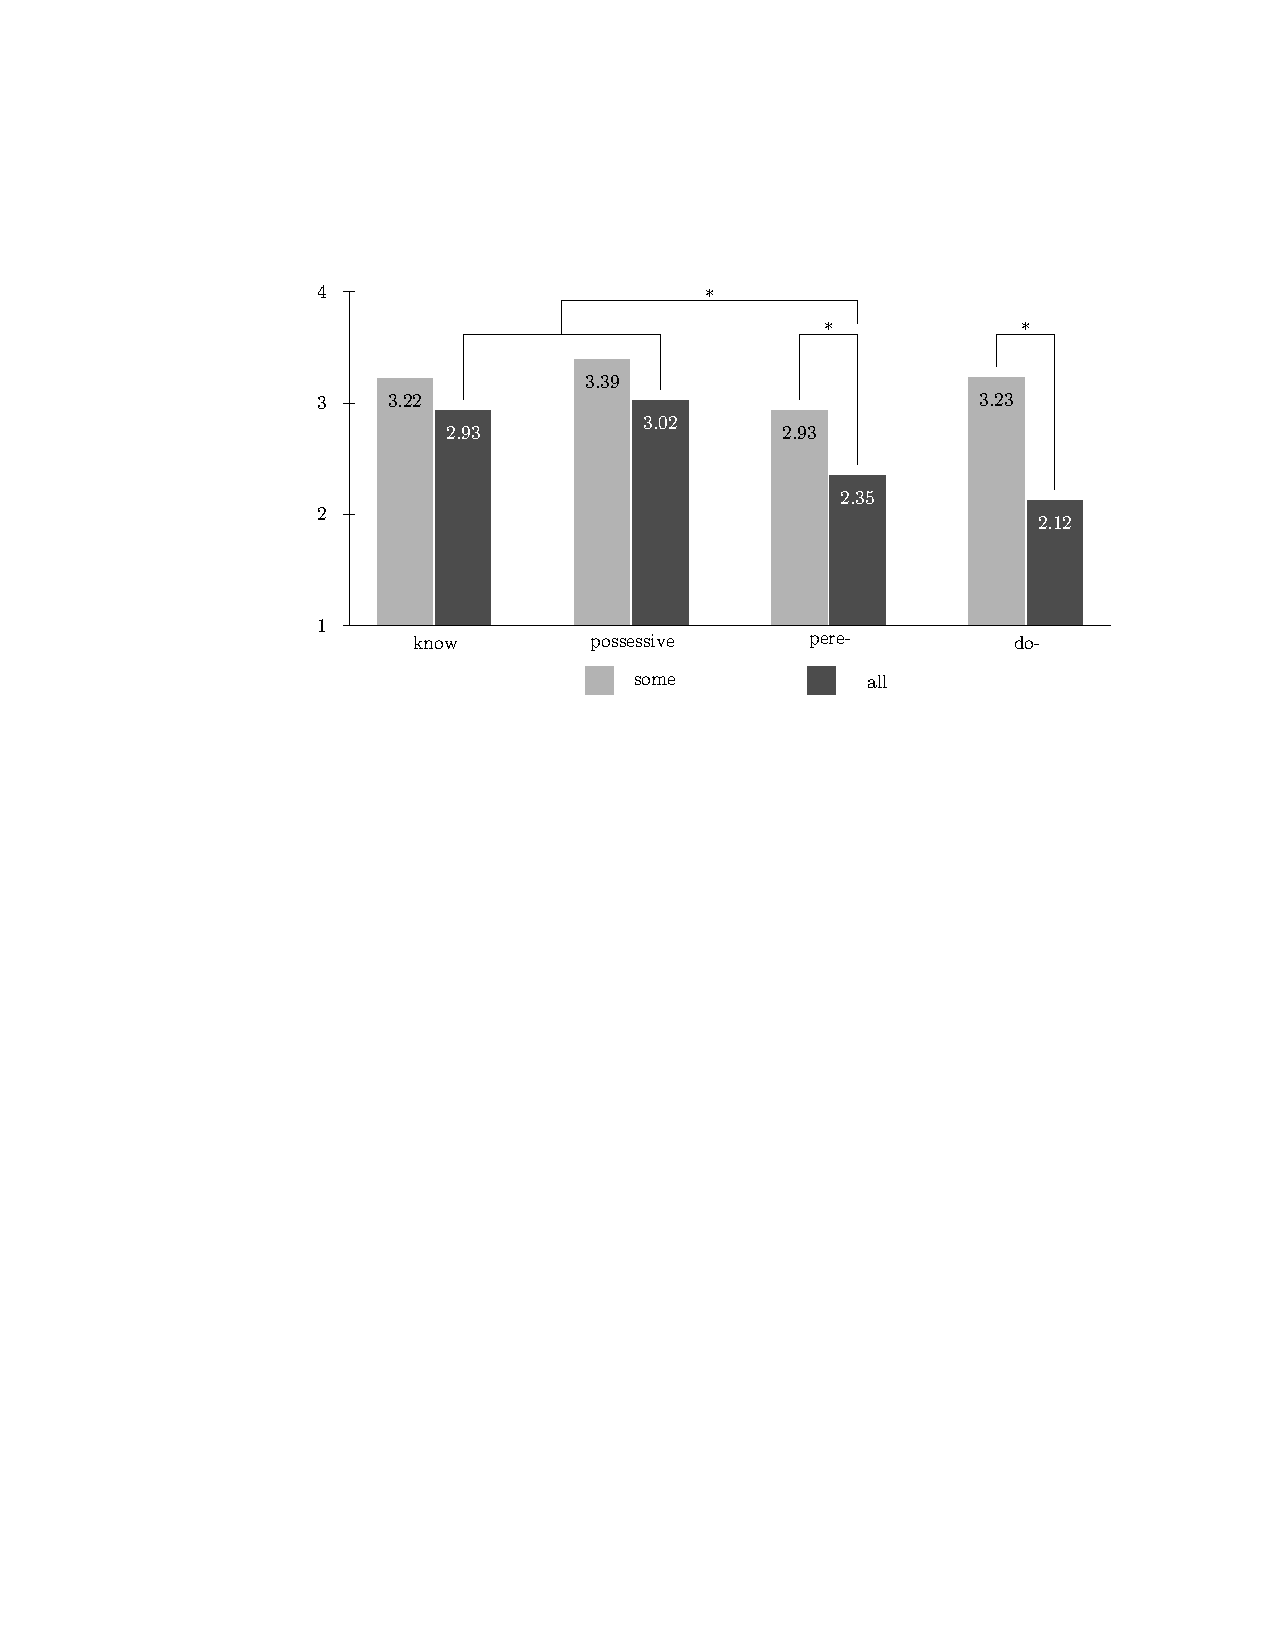
\includegraphics[width=\textwidth]{tr1.pdf}
\caption{Acceptability of existential and universal inferences for different triggers}
\label{fig:results}
\end{figure}

The main results of the questionnaire are provided in \figref{fig:results}.\footnote{Asterisks indicate significant difference.} It turned out that there is no statistically significant difference between the acceptance rates of universal and existential inferences in case of the presupposition trigger \textit{znat'} `to know' and posessive pronouns, which is in line with the results obtained in \citealt{Chemla:09}. There is, however, a statistically significant difference in the acceptance rate of universal and existential inferences in case of test items of both categories: those involving the verb with the completive prefix \textit{do-} and those with the verb prefixed with the iterative \textit{pere-} ($t$-test, $p<0.001$ in both cases). For the existential inferences, the answers ranged from ``yes'' to ``probably no'' and for the universal inferences, from ``probably yes'' to ``no'' and the overall results cannot be explained in terms of between-speaker variation. Furthermore, the difference between the acceptance rates in control and
test sentences for existential inferences was not significant, while the
difference for universal inferences was ($t$-test, $p<0.001$).

The obtained results strongly suggest that the inferences triggered by the completive prefix \textit{do-} and the iterative prefix \textit{pere-} are not of a presuppositional nature. On the other hand, the observed behaviour is compatible with a scalar implicature analysis.

\subsection{Conclusion}
The standard tests for semantic and pragmatic presuppositions show that inferences triggered by the perfective aspect of accomplishments do not behave like semantic or pragmatic presuppositions.

As for the inferences triggered by prefixes \textit{do-} and \textit{pere-}, standard tests could not be used as evidence for or against presuppositional analysis, and therefore a new testing method is used to establish their nature: a questionnaire based on results of experimental work by \citet{Chemla:09}.
The projection properties of Russian verbs containing prefixes \textit{do-} and \textit{pere-} in downward entailing contexts (under the universal quantifier \textit{no}) indicate that the projected inference behaves more like scalar implicature than like presupposition.

%\subsection{Factual Imperfective}
%Write about \cite{Gronn:04}
%In the book \cite{Boguslawski:63} the author suggests that factual uses of imperfective are just the the reductions of the sentences with the corresponding perfective verb.

\section{The overall pragmatic picture}\label{section:pragm:overall}
In Chapter~\ref{Chapter5}, I have evoked the notion of the pragmatic competition several times. In order to see how this competition works on the level of the whole prefixation system to result in the global picture, let us look at the domain of verbal meanings and see how this domain is covered with prefixed verbs. I propose that whenever the general meaning of the prefix is underspecified, the interpretation of a particular verb gets settled in the optimal way for the range of the prefixed verbs derived from one root to cover the range of meanings a speaker may want to express. The reasoning that I outline below is a first sketch of the analysis that must be tested on a wider range of examples.

First let me illustrate the flexibility of the individual prefixes. As we have discussed in Sections~\ref{subsection:semantics:na} and \ref{subsection:semantics:po}, verbs prefixed with \textit{na-} or \textit{po-} can refer to events that culminate when the expected/standard degree is reached. In addition, verbs prefixed with \textit{na-} can denote events that culminate at the degree higher than the expected degree. As for the verbs prefixed with \textit{po-}, they may refer to events that culminate without reaching the standard degree. This part of the prefixation system is complemented by the prefix \textit{pere-} that contributes the semantics of excess. Let us consider the verbs prefixed with \textit{pere-} in its excessive usage. It turns out that there is always another verb derived from the same base, that is used as a neutral perfective. Under \textit{neutral perfective} I mean either a verb that refers to an action performed until the normal/standard/appropriate degree,\footnote{These verbs would constitute aspectual pairs with the imperfective source verbs on the pair-based accounts of Russian verbal system. \citet{Janda:07a} calls such verbs Natural Perfectives. See also Chapter~\ref{Chapter2} for a discussion.} or a verb that denotes an action that lasted for some non-specified time.\footnote{Such verbs fall in the Complex Act Perfectives class in the account by \citet{Janda:07a}.} For example, if the verb \textit{gret'} `to heat' is prefixed with \textit{pere-}, the resulting verb \textit{peregret'} means `to overheat'. The same verb can be prefixed with \textit{na-} and the resulting verb \textit{nagret'} means `to warm up (until the desired temperature)'. In addition, the verb \textit{pogret'} `to heat' means warming up without necessarily reaching some particular temperature. In this case both \textit{nagret'} `to warm up'  and \textit{pogret'} `to heat' are neutral perfectives, only with respect to different scales. More pairs and triples are provided in the Table \ref{table:competition}. Let us explore them. 

\begin{sidewaystable}
\caption{Distribution of excess-denoting and neutral perfectives across verbal bases and prefixes \label{table:competition}}
\begin{tabularx}{\textwidth}{l  l  l  l  Q}
\lsptoprule
source verb& translation & ``excess'' & neutral & other competing verbs\\ \midrule
\textit{zanimat'sja} & `to study' & \textit{perezanimat'sja} & \textit{pozanimat'sja} & \\
\textit{platit'} & `to pay' & \textit{pereplatit'} & \textit{zaplatit'} & \textit{oplatit'$_{\TR}$} `to pay for smth'\\
\textit{rabotat'} & `to work' & \textit{pererabotat'} & \textit{porabotat'} & \textit{otrabotat'$_{\TR}$} `to work in compensation of smth'\\

\tablevspace
\textit{xvalit'} & `to praise' & \textit{perexvalit'} & \textit{poxvalit'} &\\
\textit{\v{z}arit'} & `to fry' & \textit{pere\v{z}arit'} & \textit{po\v{z}arit'} & \textit{pro\v{z}arit'} `to fry thoroughly,' \textit{na\v{z}arit'} `to fry a lot of'\\ 

\tablevspace
\textit{gret'} & `to heat' & \textit{peregret'} & \textit{nagret'} & \textit{pogret'} `to heat,' \textit{progret'} `to heat through'\\ 
\textit{kormit'} & `to feed' & \textit{perekormit'} & \textit{nakormit'} & \textit{pokormit'} `to feed'\\
\textit{trenirovat'} & `to train' & \textit{peretrenirovat'} & \textit{natrenirovat'} & \textit{potrenirovat'} `to train for some time'\\\lspbottomrule
\end{tabularx}
\end{sidewaystable}

The upper third of the table contains three intransitive verbs. The prefix that is used to form a neutral perfective depends on the scale lexicalised by the verb. If there is no scale except for the time scale, the prefix \textit{po-} is used. If there is a scale that allows for the attachment of the resultative \textit{za-}, it may be the option. The lines in the middle third of the table are occupied by two transitive verbs that denote events that are by default measured according to these verbs' internal scales and do not rely on the information coming from the verbal arguments. These verbs form neutral perfectives using the prefix \textit{po-.} In the bottom third the other type of transitive verbs is represented: for those verbs the standard is determined for the pairs of event types and undergoers. In such case it is the \textit{na-}prefixed verb that refers to the situation of reaching the standard. The attachment of the prefix \textit{po-} is also possible, but now the \textit{po-}prefixed verbs tend to refer to events in course of which the standard value is not reached.

What we see is that even if the range of prefixes that two verbs can attach is the same, as for the verbs \textit{\v{z}arit'} `to fry' and \textit{gret'} `to heat', the semantic contribution of these prefixes may be different. While both \textit{pere\v{z}arit'} `to burn by frying' and \textit{peregret'} `to overheat' have the meaning of excess, the role of the prefix \textit{na-} in the verbs \textit{na\v{z}arit'} `to fry a lot of' and \textit{nagret'} `to heat' seems to be not the same. In what follows we will explore a couple of verbs in detail and see how these differences in the final semantic contribution can be explained using pragmatic competition principles.

Consider the verb \textit{zimovat'} `to spend the winter'. The OSLIN database of verbal aspect provides the following list of the verbs derived from it: \textit{vyzimovat'} `to survive the winter' (usually about the plants), \textit{dozimovat'} `to spend the rest of the winter', \textit{zazimovat'} `to stay for the winter', \textit{otzimovat'} `to finish spending the winter', \textit{perezimovat'} `to spend the winter', \textit{pozimovat'} `to spend some winter time', \textit{prozimovat'} `to spend the winter time'. Examples illustrating the usage of these verbs are provided in \ref{ex:zimovat'}.

\ex.\label{ex:zimovat'}\ag.\label{ex:vyzimovat'}Vinograd ne mo\v{z}et vyzimovat' v srednej polose RSFSR.\\
grape not can.\glb{pres.sg.3} vy.winter.\glb{inf} in middle band RSFSR\\
\trans `Grape cannot survive the winter in the midland of the RSFSR.'\\\Source{= example of verb usage from \citealt{Ushakov:50}}
\bg.\label{ex:dozimovat'}Dozimuem na korable vo l'dax.\\
do.winter.\glb{pres.pl.1} on ship in ice.\glb{pl.prep}\\
\trans `We will spend the rest of the winter on a ship on the ice.'\\\Source{= example of verb usage from \citealt{Ushakov:50}}
\bg.\label{ex:zazimovat'}\`{E}kspedicija zazimovala na Novoj Zemle.\\
expedition.\glb{sg.nom} za.winter.\glb{pst.sg.f} on Novaya Zemlya\\
\trans `The expedition wintered on Novaya Zemlya.'\\\Source{= example of verb usage from \citealt{Ushakov:50}}
\bg.\label{ex:otzimovat'}Otzimovali my pervuju zimu, k vesne priez\v{z}aet Matvei\v{c}.\\
ot.winter.\glb{pst.pl} we first winter.\glb{sg.acc}, to spring pri.ride.\glb{pres.sg.3} Matveich\\
\trans `We have spent the first winter, Matveich will arrive when the spring comes.'\Source{Dmitrij Karalis. \textit{Roman s geroinej} (2001)}
\bg.\label{ex:perezimovat'}Perezimovat' v derevne.\\
pere.winter.\glb{inf} in village.\glb{sg.prep}\\
\trans `To spend the winter in a village.'\\\Source{= example of verb usage from \citealt{Ushakov:50}}
\bg.\label{ex:pozimovat'}Ix by k nam na severa, \v{c}toby pozimovali v svoix karto\v{c}nyx domikax.\\
they {} to us on north.\glb{pl.prep}, that po.winter.\glb{pst.pl} in their card house.\glb{pl.prep}\\
\trans `I would like to see them spending winter time here in the north in their houses of cards.'\Source{\url{doskapozorakomi.ru}}
\bg.\label{ex:prozimovat'}Po oby\v{c}aju togo vremeni polk na\v{s} prozimoval v odnix i tex \v{z}e kvartirax osem' zim s li\v{s}kom.\\
along custom that time regiment.\glb{sg.nom} our pro.winter.\glb{pst.sg.m} in one and that same flat.\glb{pl.prep} eight winters with over\\
\trans `According to the customs of that time our regiment spent a bit more than eight winters in the same flats.'\\\Source{T. G. \v{S}ev\v{c}enko. \textit{Kapitan\v{s}a} (1855)}

The abundance of the derivatives of the verb \textit{zimovat'} `to spend the winter' that one finds in the dictionary data, turns out to be undermined by the status of some of these verbs in the contemporary language. Two verbs from this list are barely used (\textit{vyzimovat'} `to survive the winter' and \textit{otzimovat'} `to finish spending the winter'), the verb \textit{prozimovat'} `to spend the winter time' has been used but is not common any longer (corpora examples are mostly dated with the XIX century), so we are left with four verbs that are actually encountered in text and speech: \textit{zazimovat'} that refers to the beginning of the `spending the winter' event, \textit{dozimovat'} that focuses on its end, \textit{perezimovat'} that denotes spending the time of the whole winter, and \textit{pozimovat'} that is not related to a specific portion of the winter, but to any amount of the winter time (can be part of one winter or multiple winters). With these four verbs, we see how the available prefixed verbs cover the domain of fixing different set of points: \textit{pozimovat'} `to spend some winter time' describes a finished event of staying in some particular place without imposing further restrictions on the start and the end of the stay; \textit{zazimovat'} `to stay for the winter' establishes a connection between the start of a stay in one place and the beginning of the winter; \textit{dozimovat'} `to spend the rest of the winter' fixes the end point of the stay to be related to the end of the winter; \textit{perezimovat'} `to spend the winter' relates both the start and the end points of the stay to the beginning and the end of the winter, respectively.

The question I want to answer here is why, for example, the verb \textit{pozimovat'} `to spend some winter time', that contains the prefix \textit{po-} and therefore could, from the semantics point of view, mean `to spend the whole winter', is usually not used to refer to such an event. Similarly, the verb \textit{dozimovat'} `to spend the rest of the winter' is also not used to refer to the situation of spending the whole winter despite the fact that there is no semantic restriction that would prevent it. To see how the distribution of the meanings gets established, let us first represent the different logically natural meanings that can be realised by means of the prefixed verbs. 

It is reasonable to assume that if the speaker wants to refer to a completed event of spending some winter time at a particular location, there are in principle four situations that they may want to describe (as there are only two distinguished points on the time scale in this case): the situation of spending one whole winter, the situation of spending the initial part of the winter, the situation of spending the final part of the winter, and the situation of spending some time of the winter without bounding the event duration to the duration of the winter. These four situations are presented in Table~\ref{table:zimovat}.

\begin{table}
\caption{The domain of terminated events related to spending the winter \label{table:zimovat}}
\begin{tabular}{lcc}
\lsptoprule
 & event start = winter start & event end = winter end\\
\midrule
t$_1$ & + & +\\
t$_2$ & + & \textminus\\
t$_3$ & \textminus & +\\
t$_4$ & \textminus & \textminus\\
\lspbottomrule
\end{tabular}
\end{table}

Now let us see which prefixed verbs can describe which of the situations t$_1$--t$_4$ given the restrictions in the semantics of these prefixes. As we have discussed before, for the prefix \textit{pere-} this will be the equation of both event start and event end to the start and the end points of the relevant scale. The prefix \textit{za-} necessarily equates the start point of the event with the start point of the scale, the prefix \textit{do-} only fixes the end point of the event, equating it with the end point of the relevant scale. The prefix \textit{po-}, in turn, does not restrict the positions of the start and the end points of the event with respect to the scale. In our case the scale in question is the time scale with the start and the end points associated with the start and the end of the winter.  The combination of the meanings specified in Table~\ref{table:zimovat} with the restrictions imposed by particular prefixes is shown in \figref{fig:zimovat}.

\begin{figure}
\centering
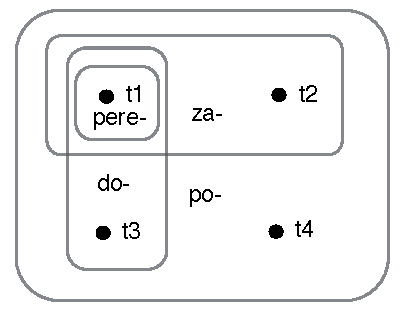
\includegraphics[scale=0.8]{dia-zimovat.pdf}
\caption{Possible interpretations of the verbs derived from \textit{zimovat'} `to spend the winter', see also Table~\ref{table:zimovat} \label{fig:zimovat}}
\end{figure}

Now pragmatic theory (e.g., Optimality Theory, henceforth OT, see \citealt{Blutner:00, vanRooy:04, Benz:11}) can be applied to the underspecified semantics representations of the prefixed perfective verbs derived from the base verb \textit{zimovat'} `to spend the winter'. As is shown in \figref{fig:zimovat}, the optimal usage of prefixed verbs would be to describe t$_1$ with the verb \textit{perezimovat'} `to spend the winter', t$_2$ and t$_3$ -- with the verbs \textit{zazimovat'} `to stay for the winter' and \textit{dozimovat'} `to spend the rest of the winter', respectively. The verb \textit{pozimovat'} `to spend some winter time' is then used in the situation t$_4$, but not in the other cases. This is exactly the distribution that is observed in the data. 

The case of the verbs that refer to the time scale only is in a way the simplest, as there are no other scales intervening. Let us now consider the verb \textit{gret'} `to heat' that is also part of Table~\ref{table:competition}. The default scale for this verb is the temperature scale. The distinguished point on this scale is the desired/appropriate temperature (let us call is t$_s$). Temperature t$_s$ depends on the direct object, as the verb \textit{gret'} `to heat' is transitive. It is also possible to talk about the other point on the scale that represents the temperature of the object at the start of the heating event, but it is not relevant for determining the space of meanings. With this we obtain three possible meanings related to the temperature scale that one may want to express: reaching a point below the distinguished point, reaching exactly the distinguished point, and reaching some point above the distinguished point. Let us call the temperature reached by the end of the heating event t$_f$. The space of meanings is presented in Table~\ref{table:gret}.

\begin{table}
\caption{The domain of terminated events related to heating \label{table:gret}}
\begin{tabular}{lccc}
\lsptoprule
 & t$_f$ $>$ t$_s$ & t$_f$ = t$_f$ & t$_f$ $<$ t$_f$\\
\midrule
t$_1$ & 1 & 0 & 0\\
t$_2$ & 0 & 1 & 0\\
t$_3$ & 0 & 0 & 1\\
\lspbottomrule
\end{tabular}
\end{table}

\begin{figure}
\centering
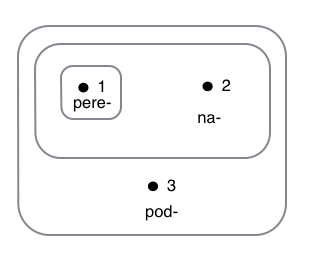
\includegraphics[scale=0.5]{dia-gret.png}
\caption{Possible interpretations of the verbs derived from \textit{gret'} `to heat', see also Table~\ref{table:gret} \label{fig:gret}}
\end{figure}

What we see in \figref{fig:gret} is the range of the meanings that certain prefixed verbs derived from the verb \textit{gret'} `to heat' may cover given the general restrictions for the semantics of these prefixes. In particular, the verb \textit{peregret'} `to overheat' can refer only to the situation of heating the object more than up to t$_s$. The verb \textit{nagret'} `to warm up' could refer to the same situation as well as to heating exactly up to the expected temperature (this temperature can be also specified via a measure phrase). The verb \textit{podogret'} `to heat to some degree' that contains the prefix \textit{pod-} (not discussed in details in this work) can refer to an event of heating that terminates with a temperature being lower than t$_s$. The verb \textit{pogret'} `to heat' can refer to any event of heating.

Applying OT to the verb-meaning pairs represented by \figref{fig:gret} results in the prediction that in the situation of overheating the verb \textit{peregret'} `to overheat' should be used. In the situation of reaching the t$_s$ the appropriate description is provided by the verb \textit{nagret'} `to heat'. The verb \textit{podogret'} `to heat to some degree' denotes exactly the situations when the temperature reached at the end of the heating event is below t$_s$. As all the relevant scenarios are covered by more specific verbs, the verb \textit{pogret'} `to heat' is used when the degree of change is not at issue and thus it is a neutral perfective.

Taking just two verbs \textit{zimovat'} `to spend the winter' and \textit{gret'} `to heat' as examples already allows us to see the source of the observed variability of the prefix interpretations. As a part of the verb \textit{pozimovat'} `to spend some winter time', the prefix \textit{po-} tends to be interpreted as restricting the portion of the winter time to be below the standard (where the standard is the duration of the winter). As a part of the verb \textit{pogret'} `to heat' the same prefix does not restrict the duration of the heating event, and the resulting verb often refers to an event of heating for the standard time. 

The description of the pragmatic competition I offer here is a first sketch. It works nicely in a number of cases I explored, but it must be tested on a wider range of verbs. Further elaboration of the approach as well as answering questions related to such architecture of the analysis goes beyond the scope of this thesis. There is a hope that the preliminary analysis I proposed here can be implemented using the computational pragmatics approach of Rational Speech Act Theory (RSA, \citealt{Franke:09, FrankGoodman:12, GoodmanStuhlmuller:13, FrankeJager:15, GoodmanFrank:16}). 

One more question that I want to mention is whether the reasoning that is used to find an optimal distribution of meanings among the available verbs is computed online or is conventionalised. The account outlined here does not favour one of the views on this process, although the status of the semantic representations for prefixes depends on the answer to this question. In future work, I plan to experimentally test whether speakers operate with the underspecified semantic representations or with conventionalised representations. 

\section{Summary}
In this chapter, we have explored inferences associated with perfective aspect and prefixes \textit{do-} and \textit{pere-}. I have provided tests that address the claim about the presence of the presuppositional component within all perfective verbs and within verbs that are derived by prefixes \textit{do-} and \textit{pere-}. For the whole class of perfectives the standard tests were enough to show that the inference in question does not have the presuppositional nature. In order to test whether prefixes \textit{do-} and \textit{pere-} trigger presuppositions I had to use a specially developed questionnaire. I then concluded that the observed inferences are better analysed as entailments and scalar implicatures (in positive and negative environments, respectively) then as presuppositions.

In the second part of the chapter, I have proposed a preliminary analysis in terms of Optimality Theory of how the prefixation system in Russian works as a whole. The idea that I plan to develop in future work is that the exact interpretation of the given verb depends on the range of competing verbs derived from the same base, while the semantic representation remains underspecified. The set of competing verbs in turn depends on the type of the scale the verb is associated with.

%\textit{igrat'} `to play.' This verb is not limited exclusively by the time scale, the other natural domain is the outcome of the playing, but the time-related domain of meanings is richer. When this verb is used intransitively, there are no specific distinguished points on the time scale, as in the case of the verb \textit{zimovat'} `to spend winter time.' The presence of a subject can contribute the appropriate time for the   \textit{pereigrat'} `to play for too long' refers to exceeding the time of playing appropriate for the subject. Together with the verbs \textit{poigrat'} `to play for some time' and \textit{proigrat' (3 \v{c}asa)} `to play continuously (for 3 hours)' the verb \textit{pereigrat'} `to play for too long' covers the domain of possible time-related meanings a speaker may want to express.

%\citet[516]{vanRooy:04} ``a linguistic convention can be seen as a behavioral phenomenon that developed through the forces of evolution.'' ``A strategy pair is successful when (i) it accounts for successful communication, and (ii) it does so with small effort.''

%TODO: bidirectional optimality theory
%TODO: Horn's division

%\section{Consequences of the proposed analysis}
%
%An important consequence of the analysis presented here is that by introducing the neutral perfectives as verbs that take as start and end points either arbitrary points on the scale or the end points of the scale, we have sold the problem of so-called ``purely perfectivizing prefixes'' \textit{(\v{c}istovidovyje pristavki)}. Such prefixes, according to Russian academic dictionaries and grammars, lack the meaning and serve just to change the aspect of the verb. is now a topic of an ungoing debate. For traditional approaches, the existence of such prefixes is a natural result of a standard procedure of identifying the meaning when writing a dictionary or grammar article: the common difference between a series of prefixed verbs versus unprefixed verbs is considered to be the meaning of the prefix.
%
%from \citet{JandaNesset:10}:\\
%The idea of “empty” prefixes, also known as “purely aspectual /
%чистовидовые”, has a long tradition in Russian linguistics (Shaxmatov:52;
%Avilova:59, Avilova:76; Tixonov:64, Tixonov:98; Forsyth:70; Vinogradov:72; Shvedova82; Certkova:96; ZaliznjakShmelev:00; Mironova:	04). 
%Some scholars have
%objected to the concept of “empty” prefixes, hypothesizing instead that there
%is conceptual overlap between prefixes and base verbs (Vey:52; vanSchooneveld:58; Isachenko:60; Timberlake:04 410–11). Though this “overlap hypothesis” is an
%attractive solution, actually proving that the prefixes are not empty has turned
%out to be one of the most long-standing and intractable problems in the field;
%Krongauz:82 labels it a “chronic” problem lacking a satisfactory solution.
%
%Natural Perfectives have the same meaning as the corresponding unprefixed
%base verb, such as растаять ‘melt’ (cf. base verb таять ‘melt’) and
%распухнуть ‘swell’ (cf. base verb пухнуть ‘swell’). Svenonius (2004a–b) and
%Ramchand (2004) refer to prefixes in such perfectives as “purely perfectivizing
%prefixes”, a term that comports well with the traditional label of
%“чистовидовая приставка.”
%
%\begin{itemize}
%\item ``Expectation 1: If the prefixes in Natural Perfectives are empty, we expect
%there to be one such prefix. '' ``Russian has, however, at least sixteen prefixes that form Natural Perfectives.'' both on p. 482
%\item Expectation 2: If the prefixes in Natural Perfectives are empty, we expect the
%prefixes to be distributed randomly. p. 482 And this is not so
%\item Expectation 3: If the prefixes in Natural Perfectives are empty, we expect the
%distribution of prefix variation to be random.
%\item Expectation 4: If the prefixes in Natural Perfectives are empty, we expect
%their assignment to borrowed verbs to be random.
%\item Expectation 5: If the prefixes in Natural Perfectives are empty, we expect
%them to stay empty.
%\end{itemize}
%
%Semantic overlap functions as a kind of camouflage making
%the meaning of the prefix hard to distinguish because it is included in the
%meaning of the verb. p. 487
%
%---------------\\
%from \citet[212]{Janda:13}
%This article focuses on the use of prefixes to form “purely aspec-­‐‑
%tual” perfective partners to simplex imperfective verbs. Prefixes used
%for this purpose are claimed by many scholars to be devoid of meaning
%(beyond marking the verb as perfective) and thus semantically “emp-­‐‑
%ty” (Šaxmatov 1952, Avilova 1959 and 1976, Tixonov 1964 and 1998,
%Forsyth 1970, Vinogradov 1972, Švedova et al. 1980, Čertkova 1996,
%Zaliznjak and Šmelev 2000, Mironova 2004). The view that prefixes are
%“empty” when they serve the function of creating aspectual pairs rests
%upon a logical argument in which we assume that meanings are like
%mathematical values. Thus if “m” is the lexical meaning of a simplex
%verb “s”, we can assume that m = s (for example, ‘write’ = pisat’). If we
%perfectivize “s” by adding a prefix “p”, the result, it is claimed, is a
%perfective verb that has the same lexical meaning as “s”, so m = p + s
%(‘write’ = napisat’). Since both “s” and “p + s” equal “m”, the value of
%“p” by this logic is necessarily zero. In other words, the prefix has no
%meaning because the lexical meaning of the verb is not changed when
%it is added. All the prefix adds is the grammatical value “+ perfective”,
%but that does not change the lexical meaning of the verb.
%
%alternative model, according to which the prefixes do bear meaning even
%when they are used to create aspectual pairs (Vey 1952, van Schoon-­‐‑
%eveld 1958, Isačenko 1960, Timberlake 2004: 410–11). Under this alter-­‐‑
%native model, it is hypothesized that the meanings of the prefixes
%overlap with the meanings of the simplex verbs. For example, one
%could say that the prefix na-­‐‑ is associated with accumulation on a sur-­‐‑
%face, and pisat’ ‘write’ is about accumulating symbols on a surface,
%motivating napisat’ ‘write’. Conceptual overlap works like camouflage,
%creating the illusion that the prefix is “empty” even though it is not.
%
%\citet{Janda:07b} suggests the term “Natural Perfectives” for verbs
%formed with “purely perfectivizing” prefixes, “Specialized Perfec-­‐‑
%tives” for verbs formed with “lexical” prefixes, and “Complex Act Per-­‐‑
%fectives” for verbs formed with “super-­‐‑lexical” prefixes.
%Janda addi-­‐‑
%tionally identifies “Single Act Perfectives” with a semelfactive mean-­‐‑
%ing (such as čixnut’ ‘sneeze once’) and shows that the types of perfec-­‐‑
%tives have distinct tendencies in terms of their semantics and deriva-­‐‑
%tional behavior.
%
%Whereas Specialized Perfectives nearly always form
%secondary imperfectives, this type of derivation is resisted to various
%degrees by the other types of perfectives. Natural Perfectives and Spe-­‐‑
%cialized Perfectives usually refer to actions that have a natural culmi-­‐‑
%nation (the completion of a document for napisat’ ‘write’ or a revision
%for perepisat’ ‘rewrite’); by contrast, Complex Act Perfectives and Sin-­‐‑
%gle Act Perfectives usually refer to actions that lack a sense of complet-­‐‑
%ability (popisat’ ‘write for a while’ is about writing without an inherent
%telos, and the lack of a culmination is inherent in sneezing as we see in
%počixat’ ‘sneeze for a while’ and čixnut’ ‘sneeze once’). Natural Perfec-­‐‑
%tives tend to behave like a closed-­‐‑class category, with a limited type
%frequency (under 2,000 verbs; see below) and relatively high token fre-­‐‑
%quency (the average median frequency of a Natural Perfective in the
%Russian National Corpus is 107), whereas other perfectives are an
%open class with unlimited type frequency (permitting occasionalisms)
%and relatively low token frequency (average median token frequency
%9.7; cf. Kuznetsova 2010). Admittedly there is no perfect dividing line
%between Natural Perfectives and other perfectives. However, there are
%very strong tendencies in this system, and the case of most verbs is
%clear despite the existence of some controversial examples.
%
%\citet[16-18]{Janda:11}
%The cluster model elaborates on the pair model in that pairs, where they exist, are either a type of cluster structure, or, more frequently, pairs are embedded in larger cluster structures containing multiple types of perfectives. In addition, the cluster model allows for structures that do not contain pairs at all. Overall, the cluster model is more accurate than the pair model in that it provides a comprehensive account of the real complexity of the Russian aspect system. 
%
%Crucial to the cluster model is the recognition of four major types of perfectives, based on their semantics and morphological behavior. The main division between the types of perfectives is motivated by Completability, since two types of perfectives are Completable and two are Non-Completable. The four types of perfectives are presented here, along with their Completability status and descriptions of the morphological behavior associated with each type:
%Natural Perfectives like napisat’ ‘write’ and svjazat’ ‘tie’ generally correspond to the perfective partners of imperfective verbs according to the pair model and share the same lexical meaning as their imperfective correlates pisat’ ‘write’ and vjazat’ ‘tie’. Natural Perfectives are strongly Completable, since they refer to the natural conclusion of a goal-oriented situation. Most Natural Perfectives are formed via prefixation of base imperfective verbs, and such Natural Perfectives often resist the formation of secondary imperfectives. Natural Perfectives can be formed from imperfectives that are either strongly Completable themselves (cf. perfective okrepnut’ from krepnut’ ‘get stronger’) or are ambiguous as to Completability (cf. perfective napisat’ from pisat’ ‘write’). There are a few base perfective verbs, usually referring to punctual events such as dat’ ‘give’ that serve as Natural Perfectives and derive the corresponding imperfective via suffixation, as in davat’ ‘give’. In addition, there are non-prototypical morphological relationships between Natural Perfectives and corresponding imperfectives, including homonymy (with bi-aspectual verbs like likvidirovat’ ‘liquidate’, where one form is both perfective and imperfective), suppletion (e.g., skazat’ ‘say’ perfective and govorit’ ‘say’ imperfective), and semi-suppletion (e.g., brosit’ ‘throw’ perfective and brosat’ ‘throw’ imperfective). 
%Specialized Perfectives like perepisat’ ‘revise’ and razvjazat’ ‘untie’ are lexically distinct from their corresponding base verbs because the prefixes direct the action in a way not inherent in the base verb. Specialized Perfectives are strongly Completable, for they refer to situations that are goal-oriented and conclude with a result (a revised manuscript or an untied knot). Specialized Perfectives can be formed from all three types of imperfectives: Completable imperfectives (such as blokirovat’ ‘block’ which forms razblokirovat’ ‘unblock’), ambiguous imperfectives (such as pisat’ ‘write’, which forms perepisat’ ‘revise’), and Non-Completable imperfectives (such as rabotat’, which forms pererabotat’ ‘revise’). There are, however, some Non-Completable imperfectives that cannot form Specialized Perfectives (such as stonat’ ‘moan’). Unlike Natural Perfectives, Specialized Perfectives nearly always form secondary imperfectives (such as perepisyvat’ ‘revise’ and razvjazyvat’ ‘untie’; but note that some verb stems resist the formation of any secondary imperfective, like kipjatit’ ‘boil’, which forms no secondary imperfective from Specialized Perfectives like perekipjatit’ ‘overboil’). 
%Complex Act Perfectives like postonat’ ‘moan for a while’ or zaprygat’ ‘start hopping’ quantize engagement in an action that lacks goal-directedness. Complex Act Perfectives focus on starting (ingressives) or stopping (terminatives) an activity or engaging in an activity for a while (delimitatives and perduratives). Since Complex Act Perfectives entail neither progress nor a result, they are strongly Non-Completable. Only imperfective base verbs that have a Non-Completable construal can form Complex Act Perfectives. Thus base verbs that are either Non-Completable (like stonat’ ‘moan’) or ambiguous for Completability (like čitat’ ‘read’) can form Complex Act Perfectives (postonat’ ‘moan for a while’ and počitat’ ‘read’ for a while), whereas strongly Completable base imperfectives tend not to form Complex Act Perfectives (such perfectives are not formed from verbs like krepnut’ ‘get stronger’ and likvidirovat’ ‘liquidate’). Complex Act Perfectives are formed by means of prefixation (primarily po-, pro-, and za-, though other prefixes such as ot-, raz- and na- also appear), and strongly resist the formation of secondary imperfectives.
%
%---------------
%
%
%However, many linguists argue against such approach and explain the fact that the meaning of such prefixes cannot be extracted not because it is not present in the prefix, but because it is also a part of the meaning contributed by the stem. This approach is advanced in such works as \cite{Isachenko:60}, \cite{Filip:00}, \cite{JandaNesset:10} and others.
%
%``the meaning of the base verb and
%prefix overlap, rendering the contribution of the prefix redundant. Redundancy,
%however, is not the same as emptiness.'' -- \citet{JandaNesset:10}
%
%
%So in addition to proposing a unified treatment for various usages of certain prefixes I want to push forward the idea of viewing the polysemy of prefix contributions as a tool for covering the domain of meanings speakers may want to express. This is in some way resembling the proposal of \citet{Janda:07a}, who subdivides perfective verbs into Natural, Complex Act, Single Act and Specialized Perfectives and then explores whether there is a certain order in which those classes get populated. As I have already noted above, some of those verbs that I classify as neutral perfectives are Natural Perfectives and some are Complex Act perfectives in the theory of \citet{Janda:07a}. For me it is important to unify those verbs in one category because this allows to see that additional inferences occur exactly in those situation when there are several prefixed verbs that could play this role.

%In section \ref{sec:pres:against}, we apply the classical tests for semantic and pragmatic presupposition to Russian data. We show that the hypothesis about the presuppositional nature of the inference triggered by perfective verbs is only applicable to a subset of perfective predicates, namely perfective accomplishments, rather than to perfectives as a whole class. Moreover,we show that this hypothesis must be rejected. When it comes to the prefixes \textit{do-} and \textit{pere-}, the tests prove to be insufficient because they do not lead to any clear judgments on the part of native speakers. In section \ref{proposal}, we present our proposal and motivate its plausibility. Section \ref{empirical} is devoted to the online questionnaire we conducted, which provides empirical evidence which supports our proposal in section \ref{proposal}.
